\section{Horn}
The purpose of the horn is to indicate an overtake when coming from behind. The horn is implemented by demand from Shell Eco Marathon. There are various demands that must followed. The most prolific of these is that the horn must emit a sound higher than 85 dB at 4 meters. For other requirements regarding the horn, see section~\ref{sec:requirements}.  

\subsection{Design}
First off, when designing the horn it was necessary to find a suitable horn, that would be able to match the requirements set forth by Shell. There were various options, but it was chosen to use an electric buzzer. This was done as it was the type of horn using the least amount of current. \\
Next up was the design of output stage. In this design it has been chosen to use a BJT transistor. It is used as a switching transistor, turning on and off according to input signal. There is a base resistance which size is defined by the h\textsubscript{fe} and the current used to supply the horn. \\
\begin{align}
	\begin{split}
		I_b &= \frac{I_c}{h_fe}
	\end{split}
\end{align}
Where $I_b$ is the current flowing into the base \\ 
$I_c$ is current flowing in the collector \\ 
$h_fe$ is the beta value of the transistor. \\

Lastly, there is going to some safety implemented. Here in the form of a diode, which supplies a path for return current when the transistor is off. This protection is mostly implemented for use with a magnetic buzzer, but it is implemented so that the PCB is prepared for many different kind of buzzers.   

\subsection{Implementation}
A full overview concerning the controls of buzzer can seen on figure underneath.

\begin{figure}[H]
	\centering
	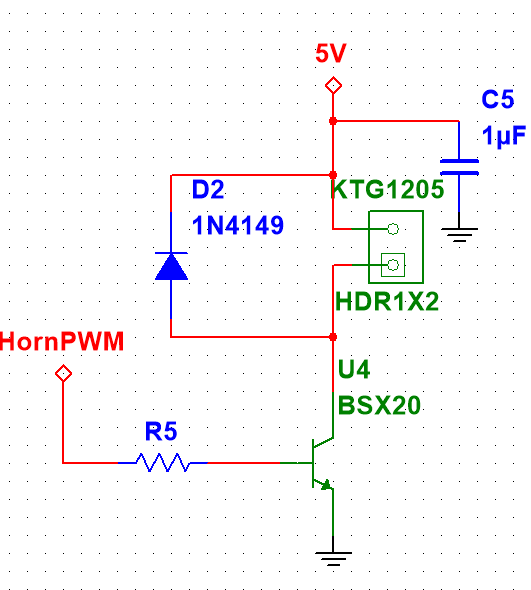
\includegraphics[width=0.7\linewidth]{Hardware/Pictures/Horn_hw}
	\caption{Horn hardware overview}
	\label{fig:Horn control}
\end{figure}

The specific transistor being used is BSX20.The datasheet \fxnote{Husk ref} for this BJT shows a minimum garaunteed $h_fe$ for these is 40 and therefore that which will be used. This makes the calculations worst case, since the used BJT probably will have a larger $h_fe$. The desired collector current will be set by the buzzer being used and will therefore vary according to that. Many of the buzzers looked upon, will draw a current of 30 mA and because it is suspected that more than one buzzer will be needed that nubmer is multiplied by 2. That leaves us with the following numbers:

$h_fe = 40 $ 

$I_c = 60 mA$

This yields 
\subsection{Unity test}
text